\documentclass[twoside]{book}

% Packages required by doxygen
\usepackage{fixltx2e}
\usepackage{calc}
\usepackage{doxygen}
\usepackage[export]{adjustbox} % also loads graphicx
\usepackage{graphicx}
\usepackage[utf8]{inputenc}
\usepackage{makeidx}
\usepackage{multicol}
\usepackage{multirow}
\PassOptionsToPackage{warn}{textcomp}
\usepackage{textcomp}
\usepackage[nointegrals]{wasysym}
\usepackage[table]{xcolor}

% Font selection
\usepackage[T1]{fontenc}
\usepackage[scaled=.90]{helvet}
\usepackage{courier}
\usepackage{amssymb}
\usepackage{sectsty}
\renewcommand{\familydefault}{\sfdefault}
\allsectionsfont{%
  \fontseries{bc}\selectfont%
  \color{darkgray}%
}
\renewcommand{\DoxyLabelFont}{%
  \fontseries{bc}\selectfont%
  \color{darkgray}%
}
\newcommand{\+}{\discretionary{\mbox{\scriptsize$\hookleftarrow$}}{}{}}

% Page & text layout
\usepackage{geometry}
\geometry{%
  a4paper,%
  top=2.5cm,%
  bottom=2.5cm,%
  left=2.5cm,%
  right=2.5cm%
}
\tolerance=750
\hfuzz=15pt
\hbadness=750
\setlength{\emergencystretch}{15pt}
\setlength{\parindent}{0cm}
\setlength{\parskip}{3ex plus 2ex minus 2ex}
\makeatletter
\renewcommand{\paragraph}{%
  \@startsection{paragraph}{4}{0ex}{-1.0ex}{1.0ex}{%
    \normalfont\normalsize\bfseries\SS@parafont%
  }%
}
\renewcommand{\subparagraph}{%
  \@startsection{subparagraph}{5}{0ex}{-1.0ex}{1.0ex}{%
    \normalfont\normalsize\bfseries\SS@subparafont%
  }%
}
\makeatother

% Headers & footers
\usepackage{fancyhdr}
\pagestyle{fancyplain}
\fancyhead[LE]{\fancyplain{}{\bfseries\thepage}}
\fancyhead[CE]{\fancyplain{}{}}
\fancyhead[RE]{\fancyplain{}{\bfseries\leftmark}}
\fancyhead[LO]{\fancyplain{}{\bfseries\rightmark}}
\fancyhead[CO]{\fancyplain{}{}}
\fancyhead[RO]{\fancyplain{}{\bfseries\thepage}}
\fancyfoot[LE]{\fancyplain{}{}}
\fancyfoot[CE]{\fancyplain{}{}}
\fancyfoot[RE]{\fancyplain{}{\bfseries\scriptsize Generated by Doxygen }}
\fancyfoot[LO]{\fancyplain{}{\bfseries\scriptsize Generated by Doxygen }}
\fancyfoot[CO]{\fancyplain{}{}}
\fancyfoot[RO]{\fancyplain{}{}}
\renewcommand{\footrulewidth}{0.4pt}
\renewcommand{\chaptermark}[1]{%
  \markboth{#1}{}%
}
\renewcommand{\sectionmark}[1]{%
  \markright{\thesection\ #1}%
}

% Indices & bibliography
\usepackage{natbib}
\usepackage[titles]{tocloft}
\setcounter{tocdepth}{3}
\setcounter{secnumdepth}{5}
\makeindex

% Hyperlinks (required, but should be loaded last)
\usepackage{ifpdf}
\ifpdf
  \usepackage[pdftex,pagebackref=true]{hyperref}
\else
  \usepackage[ps2pdf,pagebackref=true]{hyperref}
\fi
\hypersetup{%
  colorlinks=true,%
  linkcolor=blue,%
  citecolor=blue,%
  unicode%
}

% Custom commands
\newcommand{\clearemptydoublepage}{%
  \newpage{\pagestyle{empty}\cleardoublepage}%
}

\usepackage{caption}
\captionsetup{labelsep=space,justification=centering,font={bf},singlelinecheck=off,skip=4pt,position=top}

%===== C O N T E N T S =====

\begin{document}

% Titlepage & ToC
\hypersetup{pageanchor=false,
             bookmarksnumbered=true,
             pdfencoding=unicode
            }
\pagenumbering{alph}
\begin{titlepage}
\vspace*{7cm}
\begin{center}%
{\Large My Project }\\
\vspace*{1cm}
{\large Generated by Doxygen 1.8.13}\\
\end{center}
\end{titlepage}
\clearemptydoublepage
\pagenumbering{roman}
\tableofcontents
\clearemptydoublepage
\pagenumbering{arabic}
\hypersetup{pageanchor=true}

%--- Begin generated contents ---
\chapter{Hierarchical Index}
\section{Class Hierarchy}
This inheritance list is sorted roughly, but not completely, alphabetically\+:\begin{DoxyCompactList}
\item \contentsline{section}{Super\+Cool\+Class}{\pageref{class_super_cool_class}}{}
\begin{DoxyCompactList}
\item \contentsline{section}{Super\+Cool\+Class2}{\pageref{class_super_cool_class2}}{}
\end{DoxyCompactList}
\item \contentsline{section}{Vector}{\pageref{struct_vector}}{}
\end{DoxyCompactList}

\chapter{Class Index}
\section{Class List}
Here are the classes, structs, unions and interfaces with brief descriptions\+:\begin{DoxyCompactList}
\item\contentsline{section}{\hyperlink{class_super_cool_class}{Super\+Cool\+Class} }{\pageref{class_super_cool_class}}{}
\item\contentsline{section}{\hyperlink{class_super_cool_class2}{Super\+Cool\+Class2} }{\pageref{class_super_cool_class2}}{}
\item\contentsline{section}{\hyperlink{struct_vector}{Vector} }{\pageref{struct_vector}}{}
\end{DoxyCompactList}

\chapter{File Index}
\section{File List}
Here is a list of all files with brief descriptions\+:\begin{DoxyCompactList}
\item\contentsline{section}{\hyperlink{main_8cpp}{main.\+cpp} }{\pageref{main_8cpp}}{}
\item\contentsline{section}{\hyperlink{super__cool__class_8hh}{super\+\_\+cool\+\_\+class.\+hh} }{\pageref{super__cool__class_8hh}}{}
\end{DoxyCompactList}

\chapter{Class Documentation}
\hypertarget{class_super_cool_class}{}\section{Super\+Cool\+Class Class Reference}
\label{class_super_cool_class}\index{Super\+Cool\+Class@{Super\+Cool\+Class}}


{\ttfamily \#include $<$super\+\_\+cool\+\_\+class.\+hh$>$}

Inheritance diagram for Super\+Cool\+Class\+:\begin{figure}[H]
\begin{center}
\leavevmode
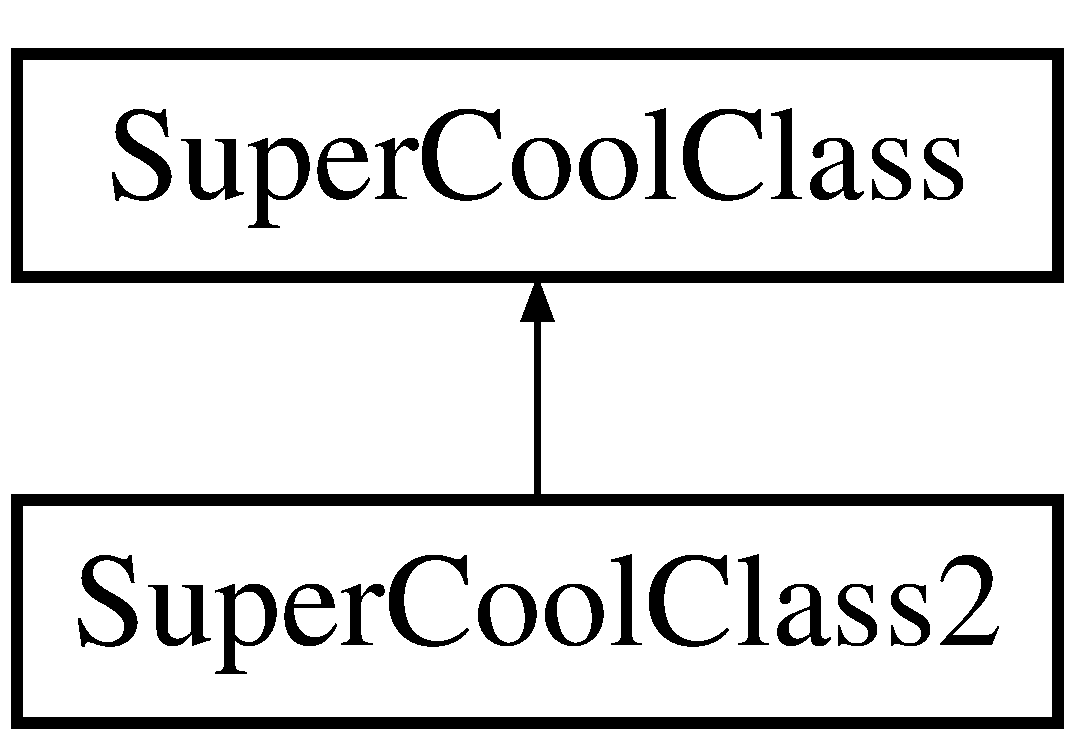
\includegraphics[height=2.000000cm]{class_super_cool_class}
\end{center}
\end{figure}
\subsection*{Public Member Functions}
\begin{DoxyCompactItemize}
\item 
\hyperlink{struct_vector}{Vector} \hyperlink{class_super_cool_class_a761c470f000de1a101a855de2d49d195}{get\+Position} (unsigned int dir)
\end{DoxyCompactItemize}
\subsection*{Protected Attributes}
\begin{DoxyCompactItemize}
\item 
int \hyperlink{class_super_cool_class_a0264bf7dc5bfe0057907102b2b5b767d}{var}
\begin{DoxyCompactList}\small\item\em A super cool variable. \end{DoxyCompactList}\item 
double \hyperlink{class_super_cool_class_a0cd88b6d83d78b0f2988647f09b28d89}{var1}
\item 
int \hyperlink{class_super_cool_class_a3aab6b04514bbac39bccd961b2ad470e}{var2}
\begin{DoxyCompactList}\small\item\em Another cool variable. \end{DoxyCompactList}\end{DoxyCompactItemize}


\subsection{Detailed Description}
This is my super cool class 

Definition at line 12 of file super\+\_\+cool\+\_\+class.\+hh.



\subsection{Member Function Documentation}
\mbox{\Hypertarget{class_super_cool_class_a761c470f000de1a101a855de2d49d195}\label{class_super_cool_class_a761c470f000de1a101a855de2d49d195}} 
\index{Super\+Cool\+Class@{Super\+Cool\+Class}!get\+Position@{get\+Position}}
\index{get\+Position@{get\+Position}!Super\+Cool\+Class@{Super\+Cool\+Class}}
\subsubsection{\texorpdfstring{get\+Position()}{getPosition()}}
{\footnotesize\ttfamily \hyperlink{struct_vector}{Vector} Super\+Cool\+Class\+::get\+Position (\begin{DoxyParamCaption}\item[{unsigned int}]{dir }\end{DoxyParamCaption})\hspace{0.3cm}{\ttfamily [inline]}}

A cool class to test dyoxigen


\begin{DoxyParams}{Parameters}
{\em dir} & \\
\hline
\end{DoxyParams}
\begin{DoxyReturn}{Returns}
a vector 
\end{DoxyReturn}


Definition at line 22 of file super\+\_\+cool\+\_\+class.\+hh.



\subsection{Member Data Documentation}
\mbox{\Hypertarget{class_super_cool_class_a0264bf7dc5bfe0057907102b2b5b767d}\label{class_super_cool_class_a0264bf7dc5bfe0057907102b2b5b767d}} 
\index{Super\+Cool\+Class@{Super\+Cool\+Class}!var@{var}}
\index{var@{var}!Super\+Cool\+Class@{Super\+Cool\+Class}}
\subsubsection{\texorpdfstring{var}{var}}
{\footnotesize\ttfamily int Super\+Cool\+Class\+::var\hspace{0.3cm}{\ttfamily [protected]}}



A super cool variable. 



Definition at line 23 of file super\+\_\+cool\+\_\+class.\+hh.

\mbox{\Hypertarget{class_super_cool_class_a0cd88b6d83d78b0f2988647f09b28d89}\label{class_super_cool_class_a0cd88b6d83d78b0f2988647f09b28d89}} 
\index{Super\+Cool\+Class@{Super\+Cool\+Class}!var1@{var1}}
\index{var1@{var1}!Super\+Cool\+Class@{Super\+Cool\+Class}}
\subsubsection{\texorpdfstring{var1}{var1}}
{\footnotesize\ttfamily double Super\+Cool\+Class\+::var1\hspace{0.3cm}{\ttfamily [protected]}}

A detailed description of a double cool variable. This description, unlike the other ones, will not appear in the protected attributes part of the dyoxigen 

Definition at line 28 of file super\+\_\+cool\+\_\+class.\+hh.

\mbox{\Hypertarget{class_super_cool_class_a3aab6b04514bbac39bccd961b2ad470e}\label{class_super_cool_class_a3aab6b04514bbac39bccd961b2ad470e}} 
\index{Super\+Cool\+Class@{Super\+Cool\+Class}!var2@{var2}}
\index{var2@{var2}!Super\+Cool\+Class@{Super\+Cool\+Class}}
\subsubsection{\texorpdfstring{var2}{var2}}
{\footnotesize\ttfamily int Super\+Cool\+Class\+::var2\hspace{0.3cm}{\ttfamily [protected]}}



Another cool variable. 



Definition at line 30 of file super\+\_\+cool\+\_\+class.\+hh.



The documentation for this class was generated from the following file\+:\begin{DoxyCompactItemize}
\item 
\hyperlink{super__cool__class_8hh}{super\+\_\+cool\+\_\+class.\+hh}\end{DoxyCompactItemize}

\hypertarget{class_super_cool_class2}{}\section{Super\+Cool\+Class2 Class Reference}
\label{class_super_cool_class2}\index{Super\+Cool\+Class2@{Super\+Cool\+Class2}}


{\ttfamily \#include $<$super\+\_\+cool\+\_\+class.\+hh$>$}

Inheritance diagram for Super\+Cool\+Class2\+:\begin{figure}[H]
\begin{center}
\leavevmode
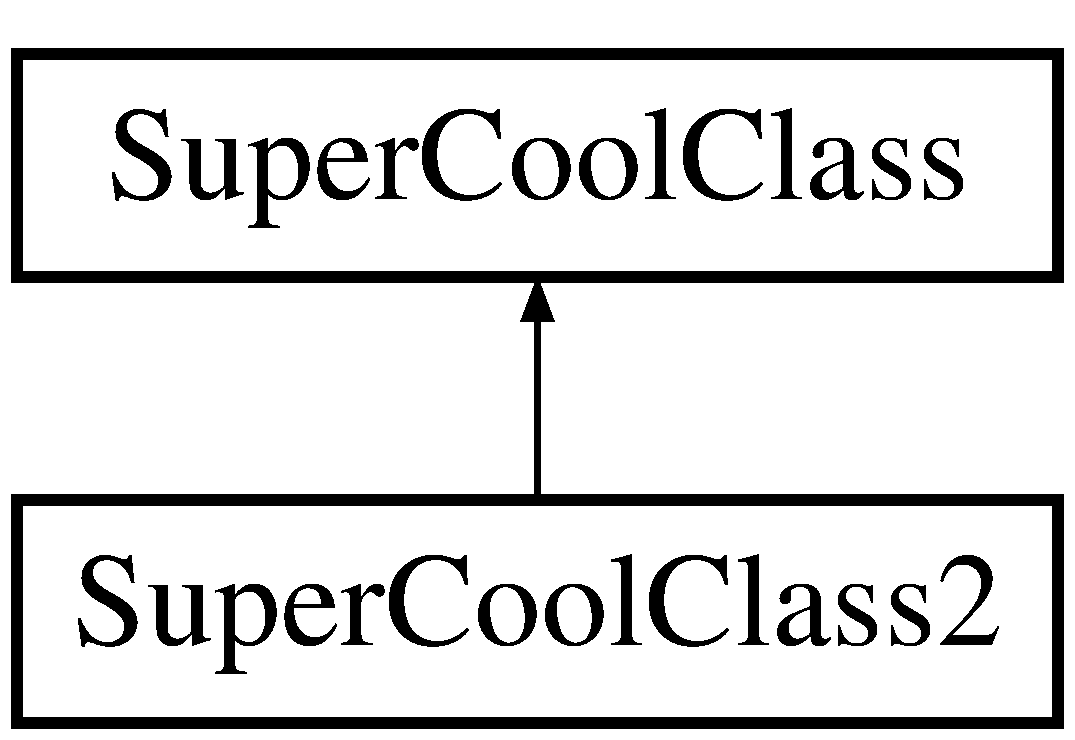
\includegraphics[height=2.000000cm]{class_super_cool_class2}
\end{center}
\end{figure}
\subsection*{Additional Inherited Members}


\subsection{Detailed Description}


Definition at line 34 of file super\+\_\+cool\+\_\+class.\+hh.



The documentation for this class was generated from the following file\+:\begin{DoxyCompactItemize}
\item 
\hyperlink{super__cool__class_8hh}{super\+\_\+cool\+\_\+class.\+hh}\end{DoxyCompactItemize}

\hypertarget{struct_vector}{}\section{Vector Struct Reference}
\label{struct_vector}\index{Vector@{Vector}}


{\ttfamily \#include $<$super\+\_\+cool\+\_\+class.\+hh$>$}

\subsection*{Public Attributes}
\begin{DoxyCompactItemize}
\item 
double \hyperlink{struct_vector_adc995472c3e3bd817a76e705f2eddc90}{val} \mbox{[}3\mbox{]}
\end{DoxyCompactItemize}


\subsection{Detailed Description}


Definition at line 2 of file super\+\_\+cool\+\_\+class.\+hh.



\subsection{Member Data Documentation}
\mbox{\Hypertarget{struct_vector_adc995472c3e3bd817a76e705f2eddc90}\label{struct_vector_adc995472c3e3bd817a76e705f2eddc90}} 
\index{Vector@{Vector}!val@{val}}
\index{val@{val}!Vector@{Vector}}
\subsubsection{\texorpdfstring{val}{val}}
{\footnotesize\ttfamily double Vector\+::val\mbox{[}3\mbox{]}}



Definition at line 4 of file super\+\_\+cool\+\_\+class.\+hh.



The documentation for this struct was generated from the following file\+:\begin{DoxyCompactItemize}
\item 
\hyperlink{super__cool__class_8hh}{super\+\_\+cool\+\_\+class.\+hh}\end{DoxyCompactItemize}

\chapter{File Documentation}
\hypertarget{main_8cpp}{}\section{main.\+cpp File Reference}
\label{main_8cpp}\index{main.\+cpp@{main.\+cpp}}
{\ttfamily \#include $<$zlib.\+h$>$}\newline
{\ttfamily \#include $<$iostream$>$}\newline
{\ttfamily \#include $<$fstream$>$}\newline
{\ttfamily \#include $<$sstream$>$}\newline
{\ttfamily \#include \char`\"{}super\+\_\+cool\+\_\+class.\+hh\char`\"{}}\newline
\subsection*{Functions}
\begin{DoxyCompactItemize}
\item 
int \hyperlink{main_8cpp_ae66f6b31b5ad750f1fe042a706a4e3d4}{main} ()
\end{DoxyCompactItemize}


\subsection{Function Documentation}
\mbox{\Hypertarget{main_8cpp_ae66f6b31b5ad750f1fe042a706a4e3d4}\label{main_8cpp_ae66f6b31b5ad750f1fe042a706a4e3d4}} 
\index{main.\+cpp@{main.\+cpp}!main@{main}}
\index{main@{main}!main.\+cpp@{main.\+cpp}}
\subsubsection{\texorpdfstring{main()}{main()}}
{\footnotesize\ttfamily int main (\begin{DoxyParamCaption}{ }\end{DoxyParamCaption})}



Definition at line 7 of file main.\+cpp.


\hypertarget{super__cool__class_8hh}{}\section{super\+\_\+cool\+\_\+class.\+hh File Reference}
\label{super__cool__class_8hh}\index{super\+\_\+cool\+\_\+class.\+hh@{super\+\_\+cool\+\_\+class.\+hh}}
\subsection*{Classes}
\begin{DoxyCompactItemize}
\item 
struct \hyperlink{struct_vector}{Vector}
\item 
class \hyperlink{class_super_cool_class}{Super\+Cool\+Class}
\item 
class \hyperlink{class_super_cool_class2}{Super\+Cool\+Class2}
\end{DoxyCompactItemize}

%--- End generated contents ---

% Index
\backmatter
\newpage
\phantomsection
\clearemptydoublepage
\addcontentsline{toc}{chapter}{Index}
\printindex

\end{document}
